\documentclass[]{article}

\usepackage{sbc2001}

\usepackage[utf8]{inputenc}
\usepackage{amssymb,amsmath}
\usepackage[portuges,brazil]{babel}
\usepackage{boxedminipage}
\usepackage{listings}
\usepackage{ifpdf}
\usepackage{longtable}
\usepackage{url}

\ifpdf
\usepackage[pdftex]{graphicx}
\else
\usepackage{graphicx}
\fi

\newcommand{\HRule}{\rule{\linewidth}{1mm}}

\begin{document}

\date{Julho 22, 2010}   

\sloppy

\title{Sistemas legados -  Migração para Novas Tecnologias : Nova plataforma de banco de dados}
\author{Marlon Gomes Lopes}

\address{
         %%Pós-Graduação \\
	 Especialização em Tecnologias Aplicadas a Sistemas de Informação com Métodos Ágeis - 4ª Edição \\
         Uniritter \\
         Porto Alegre, RS \\
         \email{marlonglopes@gmail.com}
}

\maketitle

\pagestyle{plain}
\pagenumbering{roman}


\begin{resumo}

Este artigo apresenta o detalhamento de um estudo comparativo entre bancos de dados de código fechado CACHE, SQL Server e Oracle com o objetivo de obter subsídios para a decisão de migração de plataforma de banco de dados de um sistema legado. Este estudo tem como objetivo avaliar aspectos de implementação básicos que um banco de dados deve possuir. Demonstraremos abordagens e métodos para avaliar performace bem como descrever como será conduzido o estudo comparativo. 


\end{resumo}


\begin{abstract}

This article presents the details of a comparative study between closed source databases CACHE, SQL Server, and Oracle with the aim of obtaining grants for the decision of database legacy system platform migration. This study aims to evaluate basic issues implementation of an databases. Demonstrate approaches and methods to evaluate performace and describe how the comparative study will be conducted.


\end{abstract}

\pagenumbering{arabic}
\setcounter{page}{1}

\section{Introdução}
\label{cha:introducao}
\subsection{O que é um padrão de design (\emph{Design Pattern})}
\label{sub:introducao}

Cada padrão descreve um problema que ocorre ao longo do tempo
mais de uma vez em nosso meio, e então descreve o núcleo da solução
para esse problema, de tal forma que você pode usar esta solução um milhão de vezes
mais, sem nunca fazê-lo da mesma forma duas vezes. 
Mesmo que se estivesse falando em padrões de construção de edifícios, também é verdade para padrões de construção de software orientado a objeto. Nossas soluções são expressas em termos de objetos e interfaces em vez de paredes e portas, mas no cerne dos dois tipos de padrões existe uma solução para um problema em um contexto.\cite{gamma95}

Em geral, um padrão tem quatro elementos essenciais:\cite{gamma95}

\begin{enumerate}
	\item 

O \textbf{nome do padrão} é um identificador que podemos usar para descrever um problema de \emph{design}, suas
soluções, e suas consequências em uma ou duas palavras. A nomeação de um padrão imediatamente
aumenta o nosso vocabulário de design. Ela nos permite projetar em um nível mais elevado de
abstração. Ter um vocabulário de padrões permite-nos falar sobre eles com
nossos colegas, em nossa documentação, e até mesmo para nós mesmos. Torna-se
mais fácil pensar sobre os projetos e comunicar-se com as pessoas envolvidas. Encontrar bons nomes tem sido uma das partes mais difíceis de desenvolver nosso catálogo.

	\item 


O \textbf{problema} descreve quando aplicar o padrão. Ele explica o problema
e seu contexto. Poderia descrever os problemas específicos de design tais como
como representar algoritmos como objetos. Poderia descrever classe ou
estruturas de objeto que são sintomáticas de um projeto inflexível. Às vezes, a
problema irá incluir uma lista de condições que devem ser cumpridas antes que faça
sentido de aplicar o padrão.


	\item 


A \textbf{solução} descreve os elementos que compõem o projeto, suas
relações, responsabilidades e colaborações. A solução não
descreve um determinado design concreto ou de execução, porque um padrão
é como um modelo que pode ser aplicado em muitas situações diferentes. Em vez disso,
o padrão fornece uma descrição abstrata de um problema de projeto e como
um regime geral de elementos (classes e objetos no nosso caso) resolve
ele.

	\item 


As \textbf{consequências} são os resultados da aplicação do modelo.
Quando descrevemos as decisões de design, eles são críticos para avaliar alternativas de projeto e para a compreensão
dos custos e benefícios da aplicação do modelo. As consequências para o
software são preocupação com freqüência e tempo de execução. Podem sinalizar linguagem
e questões de implementação. Uma vez que a reutilização é frequentemente um fator de
\emph{design} orientado a objeto, as conseqüências de um padrão inclui o seu impacto
sobre a flexibilidade de um sistema, extensibilidade ou portabilidade. Listando estas
conseqüências explicitamente ajuda você a compreender e avaliá-los.


\end{enumerate}

\subsection{\emph{Design Patterns} existentes}
\label{sub:designexistentes}


Os padrões hoje existentes estão divididos em três grupos:\cite{gamma95}

\begin{itemize}
	\item
		Padrões de criação (\emph{Creational patterns}) \\

		\begin{itemize}
			\item 
				\emph{Abstract factory}, Fornece uma interface para criar famílias de objetos relacionados ou dependentes sem especificar suas classes concretas.\\

			\item 
				\emph{Builder}, Separa a construção de um objeto complexo da sua representação para que
o mesmo processo de construção possa criar diferentes representações.\\
			\item 
				\emph{Factory method}, Define uma interface para criar um objeto, mas deixa as subclasses decidirem qual classe instanciar. \emph{Factory Method} permite subclasses façam a instanciação.\\

			\item 
				\emph{Prototype}, Especifica o tipo de objectos a criar usando uma instância de protótipo, e cria
novos objetos copiando este protótipo.\\

			\item 
				\emph{Singleton}, Certifica-se de que uma classe tem apenas um exemplo, e fornece um ponto global de acesso à ele.\\

		\end{itemize}

	\item
		Padrões estruturais (\emph{Structural patterns})\\
		
		\begin{itemize}
			\item \emph{Adapter}, Converte a interface de uma classe para outra interface que os clientes esperam. Este adaptador permite que classes trabalhem em conjunto, de outro modo não seria possivel por causa da incompatibilidade
interfaces.  \\
			\item \emph{Bridge}, Desacopla uma abstração de sua implementação para que as duas possam variar
de forma independente.\\

			\item \emph{Composite}, Tem o objetivo de compor objetos em estruturas de árvore para representar hierarquias parte-todo. \emph{Composite} permite que clientes tratem objetos individuais e composições de objetos
uniformemente.\\

			\item
				\emph{Decorator}, Anexa responsabilidades adicionais a um objeto dinamicamente. \emph{Decorators} fornecem uma alternativa flexível a subclasses para extensão da funcionalidade.\\

			\item \emph{Facade}, Fornece uma interface unificada para um conjunto de interfaces em um subsistema. \emph{Facade} define uma interface de alto nível que torna o subsistema mais fácil de usar.\\

			\item \emph{Flyweight}, Usa compartilhamento para suportar um grande número de objetos de forma eficiente.\\

			\item \emph{Proxy}, Proporciona um espaço para outro objeto para controlar o acesso a ele.\\


		\end{itemize}

	\item
		Padrões comportamentais (\emph{Behavioral patterns})\\

		\begin{itemize}
			\item \emph{Chain of Responsibility}, Evita o acoplamento do remetente de um pedido de seu receptor, dando a mais de um objeto a oportunidade para manipular a solicitação. Faz com que a cadeia os objetos e passe a receber pedido até que um objeto gere.\\

			\item \emph{Command}, Encapsula uma solicitação como um objeto, assim permitindo parametrizar clientes com
diferentes pedidos, cria fila ou solicitações de log e suporte às operações reversível.\\

			\item \emph{Interpreter}, Dada uma linguagem, define uma representação para sua gramática juntamente com um intérprete que usa a representação para interpretar sentenças na linguagem.\\

			\item \emph{Iterator}, Fornece uma maneira de acessar os elementos de um objeto agregado seqüencialmente sem expor sua representação subjacente.\\

			\item \emph{Mediator}, Define um objeto que encapsula como um conjunto de objetos \emph{interact.Mediator} promove acoplamento, mantendo os objetos de cada EPI referindo explicitamente outros, e ele permite que você varie sua interação de forma independente.\\


			\item \emph{Memento}, Sem violar o encapsulamento, captura e externaliza o estado de um \emph{object sinternal} para que o objeto pode ser restaurado para este estado mais tarde. \\

			\item \emph{Observer}, Define uma dependência um-para-muitos entre objetos de modo que quando um objeto muda de estado, todos seus dependentes sejam notificados e atualizados automaticamente.\\

			\item \emph{State}, Permite que um objeto altere seu comportamento quando seu estado interno muda.\\
			
			\item \emph{Strategy}, Define uma família de algoritmos, encapsula cada um, e torna-os intercambiáveis.
Esta estratégia permite que o algoritmo pode variar independentemente do cliente que usá-lo.\\


			\item \emph{Template Method}, Define o esqueleto de um algoritmo numa operação, adiando alguns passos para as subclasses. Permite que subclasses redefinam certos passos de um algoritmo sem alterar a estrutura do algoritmo.\\

			\item \emph{Visitor}, Representa uma operação a ser realizada sobre os elementos de uma estrutura de objetos. Permite que você defina uma nova operação sem alterar as classes dos elementos em que opera.\\



		\end{itemize}

\end{itemize}

Estes são os padrões mais comumente utilizados, neste trabalho será detalhado o Padrão de criação \emph{Factory Method}, tambem conhecido como \emph{Virtual Constructor} (Construtor virtual).


\section{Argumentos para Migração}
\label{cha:argumentos}
Até meados dos anos 60, os dados eram mantidos aleatoriamente em arquivos, geralmente como partes integrantes da aplicação. A partir dessa época, surgiram os primeiros Sistemas Gerenciadores de Bancos de Dados (SGBDs) comerciais, provendo armazenamento dos dados de forma independente da aplicação, contudo, sem mecanismos de acesso eficientes. \cite{boscarioli2006} 

Um percentual significativo dos sistemas de informação ainda hoje usados foram desenvolvidos ao longo dos últimos vinte anos e não utilizam bancos de dados relacionais. Os dados destes sistemas estão armazenados em arquivos de linguagens de terceira geração, como Basic, COBOL, MUMPS e outras, ou então em bancos de dados da era pré-relacional, como IMS, ADABAS, DMS-II e os SGBD do tipo CODASYL (IDMS, IDS/2,...). \cite{heuser2001projeto}

Existe um grande número de tecnologias de gerenciamento de dados de grande porte. Essas tecnologias vão de sistemas de arquivos texto até sistemas relacionais de banco de dados de grande porte. 

Independentemente do tipo de solução que uma empresa decide utilizar, o que na em certa época era a melhor solução hoje pode estar desatualizado. Nestes casos, deve ser estudado uma mudança de plataforma de armazenamento de dados. 

Existem muitos motivos para que uma empresa decida migrar de plataforma de banco de dados, e antes de migrar estas empresas devem escolher cuidadosamente a tecnologia que atenda as necessidades atuais e que atenderá as suas necessidades o maior tempo possível após a migração. 

A migração de plataforma de armazenamento é um assunto muito sério. Os dados da empresa significam conhecimento. Todos os projetos de migração embutem um nível de risco alto. Entretanto, um projeto de migração bem planejado e corretamente executado pode fazer com que a empresa possa prover soluções melhores com acesso aos dados de maneira mais rápida e otimizada.

Um sistema legado, no contexto organizacional possui vários componentes para uma discussão técnica, mas, podemos considerar o seguinte: 

- O hardware de Apoio na maioria dos sistemas obsoletos o hardware é antigo, e não existe mais fornecedor e a manutenção é cara.

- O Software de apoio, como sistema operacional, compiladores, ferramentas, etc também podem estar desatualizado. 

- O software de aplicação em sistema legado não é um único programa de aplicação, inclui geralmente vários programas. Começa com pequenos projetos de pequeno porte e ao longo do tempo varias alterações e inclusões são implementadas tornando o sistema legado muito robusto e de difícil manutenção, e muitas vezes os programadores originais nao estão mais presentes.

- Os  dados de aplicação em muitos sistemas legados possui um imenso volume de dados que se acumulou com o passar do tempo de existência do sistema. Estes dados podem conter inconsistências e muitas vezes os dados estao duplicados em diferentes bases, em função das novas implementações feitas por diferentes programadores que desconheciam o sistema totalmente.

- As regras ou processos de negócio as informações sobre os processos internos da organização, codificadas em uma linguagem e espalhadas pelos programas que fazem parte do sistema. Essas regras na maioria das vezes não estao documentadas, sendo do conhecimento tácito de gerentes, analistas e programadores antigos. Os novos sistemas dificilmente reproduzirão essas regras.

Outros fatores não menos importantes como a falta de suporte, descontinuação do banco de dados, descontinuação da ferramenta de desenvolvimento, não homologação do banco de dados para sistemas operacionais atuais. 

Todos estes motivos reforçam que a integração apenas não é suficiente, pois novos hardwares exitem atualização de sistema operacional e os novos sistemas operacionais não suportam a ferramenta de BD Legado. Logo é necessário a migração total de plataforma, Banco de Dados e Linguagem de Programação.


\section{Implicações  da migração de plataforma de Banco de dados}
\label{cha:implicacoes}
Conforme mensionado anteriormente, um projeto de migração de plataforma de banco de dados é um assunto muito sério e deve ser realizado com bastante cuidado, levando em consideração os domínios de negocio existentes na empresa. A migração de dados é classificada em três níveis, conforme o trabalho necessário. Estes três níveis determinam a quantidade de trabalho e os elementos envolvidos na migração.

Migração de nível um inclui apenas o esquema ou definições de dados, e os dados em si. O necessário mais comum para uma migração de nível um, é quando o aplicativo esta usando uma interface que existe tanto na plataforma de banco de dados antigo quanto no novo. Além disso, o suporte a essa interface é idêntico nos dois sistemas. Não se esta usando nenhum recurso especial do banco de dados anterior. Portanto é necessário migrar somente as definição de dados e os dados em si. Também é necessário algum trabalho de migração, mas, uma vez que os dados tenham sido migrados, a aplicação estará funcionando.

Uma migração de nível dois inclui o esquema de dados e algumas alterações do código fonte, este nível pode ser visto como extensão do nível um. Imagine uma migração de nível um onde são usadas diferentes versões da mesma interface no banco de dados antigo e no novo. Neste caso migrar apenas o esquema e os dados não faz que o aplicativo funcione completamente; é necessário analisar as diferenças entre as versões. Uma vez que essas diferenças tenham sido identificadas, pode se alterar o código para que o aplicativo funcione com o banco de dados novo.

Uma migração de nível três é diferente dos dois anteriores. Nos níveis anteriores o único objetivo da migração é alterar o sistema de armazenamento de dados, isto é, fazer com que o aplicativo funcione com o novo banco de dados. Em uma migração de nível três a maioria do aplicativo é reescrito.

Para migração de uma plataforma muito ultrapassada para uma atual é necessário uma migração de nível três pois o sistema de armazenamento legado é muitas vezes em forma de arquivo ou não relacional. Os Bancos de dados chamados relacionais são os chamados atuais. Existem bancos chamados Pós-relacionais pois uma nova característica abordade hoje em dia é o mapeamento Objeto Relacional, e os chamados Bancos de Dados Orientados a Objeto implementam essa características.

Uma migração de nível três é uma medida extema e tem dois objetivos. Primeiro, como nas outras duas migrações, alterar o sistema de armazenamento de dados para uma nova plataforma. Segundo uma migração de nível três significa alterar a camada de acesso a dados de maneira que o aplicativo use recursos específicos no novo banco de dados. A migração de nível três representa maior custo e maior risco. Entretando, os benefícios do melhor desempenho e administração fazem que o trabalho e o custo faça valer a pena.



\section{Abordagens para Migração }
\label{cha:abordagens}
A migração total de um sistema legado envolve, pensar em banco de dados relacionais ou orientados a objeto, ferramenta de desenvolvimento modernas , segurança (interfaces web), servidores mais robustos, treinamento da equipe de desenvolvimento (métodos novos de desenvolvimento, linguagem, acesso aos dados), treinamento da equipe de suporte ao ambiente (DBA, Servidores), reestruturação da rede de suporte a  aplicação. Treinamento dos usuários para as novas interfaces. Gestão de Mudança. 

Deve ser levado em consideração a construção do modelo conceitual da base de dados legada pensando na migração do banco de dados para
uma nova plataforma de implementação, por exemplo usando um SGBD relacional. A disponibilidade de uma documentação abstrata, na forma de um modelo conceitual dos dados do sistema existente, pode acelerar em muito o processo de migração, pois permite encurtar a etapa de modelagem de dados da novo banco de dados. \cite{heuser2001projeto}

Na busca de migrar os sistemas legados, e avaliar qual plataforma melhor se adequa melhor as necessidades de uma empresa que visa estabilidade e performace em um novo ambiente, e nesse ambiente qual banco de dados servirá melhor as necessidades das aplicações desenvolvidas em determinados domínios de aplicação. 

Para tal propósito descreveremos uma maneira de conduzir um estudo comparativo de aspéctos básicos de implementação entre os SGBD CACHE, SQL Server e Oracle.



\section{Trabalhos anteriores}
\label{cha:trabs}
Recentemente, foram publicados trabalhos de criação e aperfeiçoamento de benchmarks. Um dos principais motivos é a restrição imposta pela “cláusula DeWitt” \cite{moranb}, que proíbe a realização de testes em bancos de dados comerciais sem a prévia autorização do fabricante. Em razão disso, vários benchmarks foram construídos para comparar o desempenho de SGBD de código aberto: DBT-2
\cite{osdl}, TPCC-UVA \cite{hernandez02} e OSDB \cite{osdb}. Os dois primeiros utilizam uma carga de trabalho OLTP similar a do consagrado benchmark TPC-C, da TPCTM (Transaction Processing Performance Council) \cite{tpc}. O benchmark TPC-C é a principal referência no mundo quando se trata de desempenho de sistemas computacionais. 

OLTP é um acrônimo de \emph{Online Transaction Processing} ou Processamento de transações em tempo-real. São sistemas que se encarregam de registrar todas as transações contidas em uma determinada operação organizacional. Por exemplo: sistema de transações bancárias que registra todas as operações efetuadas em um banco, caixas de multibanco, reservas de viagens ou hotel nn-line, Cartões de Crédito.

A maioria dos resultados comparando o desempenho de SGBD de código aberto foi produzida através de uma ampla variedade de benchmarks e estes resultados são muitas vezes contraditórios e tendenciosos.

Neste trabalho o objetivo é apenas auxiliar na decisão de migração de plataforma, e não apontar falhas ou publicar os resultados com fins comerciais.

\subsection{O Benchmark OSDB}
\label{cha:osdb}
O benchmark OSDB (\emph{Open Source Database Benchmark}) foi criado com o objetivo
inicial de avaliar a taxa de I/O e o poder de processamento da plataforma GNU
Linux/Alpha. Sua implementação é baseada no benchmark AS3AP, diferindo em alguns
aspectos: quantidade de métricas retornadas e número de módulos. Enquanto a análise
dos resultados gerados pelo benchmark AS3AP baseia-se em uma única métrica
(tamanho máximo do banco de dados suficiente para completar o teste em menos de 12
horas), o OSDB possibilita a comparação através de outras métricas: tempo de resposta
das consultas e número de linhas retornadas por segundo.

Este benchmark é dividido em três módulos: carga e estrutura, mono-usuário
e multi-usuário. O módulo de carga e estrutura inclui a criação e carga de tabelas a
partir de dados armazenados em arquivos texto, além da criação de índices clusterizados
e não-clusterizados (apenas B-tree). No módulo mono-usuário é testado o desempenho
de seleções, junções, projeções, agregações e atualizações. A ordem de execução das
consultas é definida de forma a não favorecer a utilização de dados em cache.

No módulo multi-usuário, os testes simulam perfis de carga de trabalho
diferentes. Para cada tipo, um determinado número de processos é executado
concorrentemente, simulando uma massa de usuários conectados. A quantidade de
usuários é um quarto do tamanho do banco de dados. Os perfis de carga de trabalho
incluem: (i) perfil OLTP, considerando a base de dados de 512MB, 127 usuários
executam operações de atualização em uma única tabela. O outro usuário executa um
conjunto de 08 (oito) consultas pré-definidas sobre uma mesma tabela; (ii) perfil misto,
01 (um) usuário executa um conjunto de operações incluindo atualizações e consultas,
enquanto que os demais executam o conjunto de consultas do perfil OLTP.

Neste trabalho será utilizado um esquema de execução alternativo, para simplificar o trabalho de implementação e execução dos testes.




\section{Esquema de Execução do estudo comparativo}
\label{cha:esquema}
\subsection{Metodologia}
\label{cha:subsecmetodologia}

Será definido um estudo comparativo para avaliação de performance entre SGBDs de código fechado: Oracle, SQL Server e CACHE. A implementação será feita utilizando a linguagem C{\#} .NET.

\subsection{Definição do esquema de dados}
\label{cha:sub1esquema}


\begin{figure}[ht!]
	\begin{center}
		%%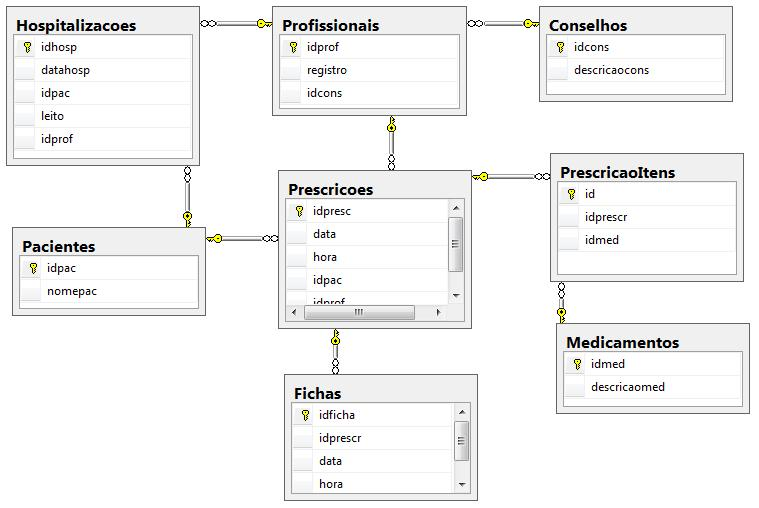
\includegraphics[width=10in,height=6in]{esquema.jpg}
		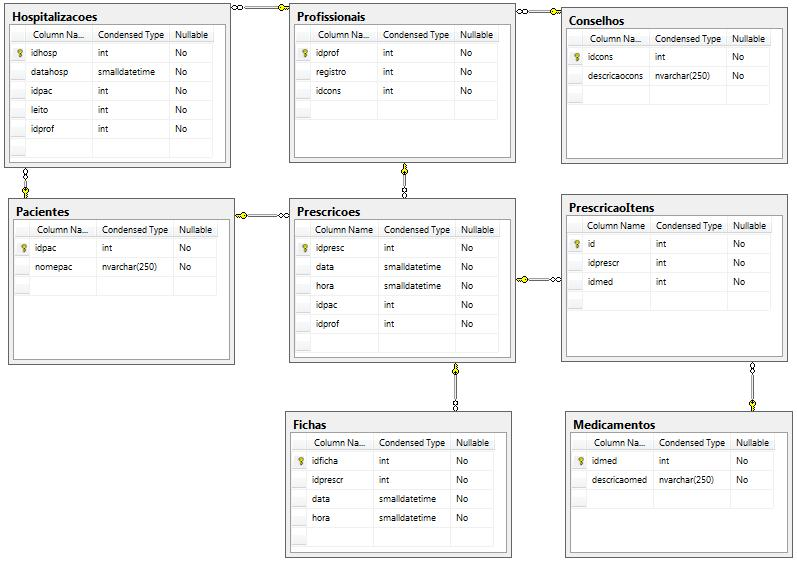
\includegraphics[scale=0.7]{esquema2.jpg}
		\caption{\label{esquema} Base de dados para execução dos testes}		
	\end{center}
\end{figure}


O esquema de dados é o conjunto de descrições que definem os tipos de dados e sua organização para o sistema de gerenciamento de banco de dados. Podem existir muitos tipos diferentes de dados, dependendo da complexidade do banco de dados.
Mesmo os sistemas de banco de dados mais simples diferenciam dados numéricos e de texto. Em bancos de dados mais
complexos, o esquema diferencia níveis de dados numéricos, além de identificar outras características dos dados.

Ao migrar o banco de dados, o esquema pode ser um desafio importante. É necessário mapear os tipos de dados do banco
de dados antigo para os tipos de dados do novo sistema de banco de dados. Eles não precisam ter o mesmo nome, mas
devem ter a mesma função. Por exemplo, se voce não mapear os tipos de dados corretamente na migração do banco de dados, podem ocorrer resultados imprevisíveis nas buscas, pior ainda, dados podem ser danificados ou perdidos.

O esquema também pode indicar relações entre tabelas. Estas relações definem a integridade referencial. Integridade referencial é uma das áreas problemáticas em gerenciamento de banco de dados, principamente se os usuarios que acessam os dados não conhecem as definições de referencias e não respeitam tais regras, para isso um bom sistema gerenciador de banco de dados deve implementar um bom mecanismo de verificação de integridade referencial.

Quanto a integridado de dados, um problema encontrado em varios bancos de dados antigos é a falta de tipagem nos dados armazenados, tornando a migração mais lenta pois é necessário a verificação dos tipos de dados nas tabelas do banco novo.

Para avaliação de performace será criado um esquema de dados de média complexidade para avaliar os aspectos necessários em um bom 
sistema de banco de dados, a figura \ref{esquema} ilustra o esquema de dados.

\subsection{Esquema de Execução do estudo comparativo}
\label{cha:sub2esquema}

Serão definidas oito tabelas relacionadas e com campos de tipos diferentes para avaliar os diferentes requisitos referêntes a intergridade dos dados e referêntes a ralacionamentos entre as tabelas.

O esquema de execução de testes consiste em estabelecer conexão com o banco de dados, marcar tempo de inicio, executar as inserções ou consultas, liberar conexão, e marcar tempo final. Nesse tempo serão executados e avaliados os seguintes testes:

- Teste de integridade de dados: 

O teste deve verificar o quanto o SGDB  controla automaticamente a integridade dos diversos tipos de dados necessários ao modelo de dados definido. O teste constitui em definir os tipos de dados de cada atributo de cada tabela e verificar a garantia de integridade dos dados;

- Teste de integridade referencial:

O teste deve verificar o nível de controle de integridade em relação a inclusão, alteração e remoção de dados de tabelas que estão relacionadas com outras tabelas.

- Teste de integridade de chave primaria:

O teste deve verificar a integridade com relação a unicidade de chaves primarias nas tabelas.

- Teste de consistência de dados:

O teste deve verificar o controle que o SGBD tem sobre os tipos de dados que fornece. O presente teste é decorrência do primeiro visto que a garantia de integridade dos dados afeta profundamente a garantia de consistência.

- Teste de performance com utilização de tabelas comuns solitárias:

O teste deve verificar se o tempo de armazenamento e recuperação de informações utilizando somente dados do tipo texto e ou numéricos em tabelas sem relacionamento é satisfatório.

- Teste de performance com utilização de tabelas com relacionamentos:

O teste deve verificar o tempo de armazenamento e recuperação de informações utilizando somente dados do tipo texto e ou numéricos em tabelas um ou mais relacionamentos.

- Teste de acesso concorrente:

O teste deve verificar a performance do sistema variando a quantidade de usuários acessando simultâneamente os dados.

A Execução dos testes será realizada remotamente e localmente, com o objetivo de avaliar tambem influências de uma rede no estabelecimento da conexão.

\subsection{Bancos de dados}
\label{cha:conhecendo}

\subsubsection{SQL Server} 

O SQL Server é um SGBD (sistema gerenciador de Banco de dados) relacional criado pela Microsof. É um Banco de dados robusto e usado por sistemas corporativos dos mais diversos portes.

É um banco de dados projetado para ser executado em plataformas que vão de laptops a servidores multiprocessador de grande porte. SQL Server é comumente usado como o sistema de infra-estrutura para sites e CRMs das empresas e pode suportar milhares de usuários simultâneos.

SQL Server vem com uma série de ferramentas para ajudá-lo com o seu banco de dados e administração de tarefas de programação.

SQL Server é muito mais robusta e escalável que um sistema de gestão de dados desktop como o Microsoft Access. Quem já tentou usar o Access como um back-end para um site provavelmente deve estar familiarizado com os erros que foram gerados quando muitos usuários tentaram acessar o banco de dados!

Embora o SQL Server também pode ser executado como um sistema de banco de dados desktop, é mais comumente usado como um sistema de banco de dados do servidor. \cite{sqlserver}

\subsubsection{Oracle}

O Oracle é um SGBD que surgiu no fim dos anos 70. O SGBD da Oracle é líder de mercado. O Oracle 9i foi pioneiro no suporte ao modelo web. O Oracle 10g, mais recente, se baseia na tecnologia de grid. Recentemente fora lançado o Oracle 11g que veio com melhorias em relação ao Oracle 10g.

Além da base de dados, a Oracle desenvolve uma suíte de desenvolvimento chamada de Oracle Developer Suite, utilizada na construção de programas de computador que interagem com a sua base de dados.

A Oracle também criou a linguagem de programação PL/SQL, utilizada no processamento de transações. \cite{oracle}

\subsubsection{Caché} 

Caché é um sistema de gerenciamento de banco de dados proprietário, produzido pela InterSystems, baseado na Tecnologia M.
A empresa descreve o banco como pós-relacional, e afirma que: oferece uma visão relacional e orientada a objetos dos mesmos dados, sem necessidade de mapeamentos ou redundância.

A arquitetura unificada do Caché suporta aplicativos orientados a objeto e relacionais utilizando SQL ANSI.

O Caché permite rápido desenvolvimento de aplicações Web, processamento transacional de alta performance, escalabilidade maciça, e consultas em tempo real de dados transacionais, além de baixíssimas necessidades de manutenção

Caché suporta diversas linguagem de programação, entre elas ObjectScript, um superconjunto funcional da linguagem M (Padrão ANSI para a linguagem MUMPS). Por motivos de mercado, a empresa prefere manter o produto Caché afastado desse nome. Os principais clientes de Caché são hospitais e financeiras americanos.

Na prática, Caché é a evolução a longo prazo da tecnologia M. Seu desempenho é considerado por muitos superior ao de SGDBRs tradicionais.

A visão pós-relacional de Caché também pode ser vista como uma visão pré-relacional e atualmente seria melhor descrita como uma visão não-relacional já que internamente Caché guarda seus dados em matrizes multi-dimensionais capazes de carregar dados estruturados hierarquicamente. Curiosamente, a tecnologia adequada para modelo de dados hierárquico sobreviveu e a total dominação do modelo relacional no mercado e hoje apresenta uma estrutura que pode ser, pelo menos em algumas aplicações, mais adequada para guardar objetos ou dados em XML.

O caché suporta modelagem de dados relacional ou orientado a objetos. \cite{cache}

\subsection{Testes com conexao com o Banco}
\label{cha:conexao}

\subsubsection{SQL Server}

Existem inúmeras formas de estrabelecer conexao com o banco, tudo depende da aplicação, existem maneiras standard de conexão que não fornecem muita segurança e existem mecanismos mais sofisticados de estabelecer conexão de maneira muito segura, abaixo alguns exemplos:

\scriptsize

\begin{verbatim}

Standard Security:

Data Source=myServerAddress;Initial Catalog=myDataBase;User Id=myUsername;Password=myPassword;

Standard Security alternative syntax

Server=myServerAddress;Database=myDataBase;User ID=myUsername;Password=myPassword;Trusted_Connection=False;

Trusted Connection:

Data Source=myServerAddress;Initial Catalog=myDataBase;Integrated Security=SSPI;

Trusted Connection alternative syntax

Server=myServerAddress;Database=myDataBase;Trusted_Connection=True;

\end{verbatim}

\normalsize

Será avaliada a string de conexão que estabelece conexão com o banco no menor tempo possível. \cite{sqlstring}

\subsubsection{Oracle}

Existem variadas formas de se estabelecer conexão com um Banco Oracle, assim como o SQL Server, utilizando objetos que recebem uma string de conexão, assim sendo tambem será testada que tipo de conexão é mais rapida. Abaixo seguem alguns exemplos.

\scriptsize

\begin{verbatim}

Using TNS
Data Source=TORCL;User Id=myUsername;Password=myPassword;

Using integrated security
Data Source=TORCL;Integrated Security=SSPI;

Using ODP.NET without tnsnames.ora
Data Source=(DESCRIPTION=(ADDRESS_LIST=(ADDRESS=(PROTOCOL=TCP)(HOST=MyHost)(PORT=MyPort)))
(CONNECT_DATA=(SERVER=DEDICATED)(SERVICE_NAME=MyOracleSID)))
;User Id=myUsername;Password=myPassword;

\end{verbatim}

\normalsize

Será avaliada a string de conexão que estabelece conexão com o banco no menor tempo possível. \cite{orastring}

\subsubsection{Caché}

\scriptsize
\begin{verbatim}

Standard
DRIVER={InterSystems ODBC};SERVER=myServerAddress;DATABASE=myDataBase;UID=myUsername;
PWD=myPassword;

Specifying port
DRIVER={InterSystems ODBC};SERVER=myServerAddress;PORT=12345;DATABASE=myDataBase; UID=myUsername;
PWD=myPassword;
 
Specifying protocol
DRIVER={InterSystems ODBC};SERVER=myServerAddress;PORT=12345;DATABASE=myDataBase;PROTOCOL=TCP;
STATIC CURSORS=1;UID=myUsername;PWD=myPassword;

\end{verbatim}

\normalsize

Será avaliada a string de conexão que estabelece conexão com o banco no menor tempo possível. \cite{cacstring}



\subsection{Testes de integridade de dados ou de domínio}
\label{cha:integridade}


Quando falamos em integridade, pensamos em proteção contra hackers e ataques do gênero, ou até mesmo backup, mas a integridade começa em um nível muito mais baixo que isto, começa na criação e projeto do banco de dados.

Integridade de domínio nada mais é do que a integridade do campo como o tipo de dados correto, se permite null ou not null, defaults, checks constraints, estes mecanismos foram criados para dar integridade aos campos. Os tipos de dados também são caracterizados como integridade de domínio, se o tipo de dado estiver incorreto, ou com mais posições que o necessário, pode haver ali um risco que quebre a integridade. O check aqui é em nível de campo apenas por exemplo: Tenho um campo Meses e quero que entre valores de 1 até 12 somente.

No estudo que será realizado testes quanto aos tipos de dados criados nas tabelas, serão executadas tentativas de inserir dados não compatíveis com os dados definidos nas tabelas, será avaliado que tipo de resposta o banco retorna e o tempo de resposta do banco de dados quando existir tentativas de inserção de dados de domínios diferentes.

\subsection{Testes de integridade referencial}
\label{cha:intref}

A integridade referencial é mais conhecida, são as \emph{Foreign Keys}, nada mais é que eu aceitar valores em minha entidade que estão em outra entidade, isto é possível a partir da integridade de entidade, eu apenas consigo criar \emph{Foreign Keys} a partir de uma \emph{Primary Key} ou uma \emph{Unique}, a integridade referencial consiste também em check em nível de tabela e não em nível de campo, no ato da criação da tabela crio um check, por exemplo:

Tenho uma tabela com 2 campos Medico1, Medico2, e quero que um dos campos sempre seja preenchido não importa qual, para isto preciso de um check em nível de tabela.

Segue tabela de tipos de integridade :

\begin{center}
	\begin{tabular}{ll}
		Tipos de Integridade & Tipo de constraint \\
		Dominio & DEFAULT, CHECK, REFERENCIAL \\
		Entidade & PRIMARY KEY, UNIQUE \\
		Referencial & FOREIGN KEY, CHECK \\
	\end{tabular}
	\captionof{table}{Tipos de integridade e constraints}
	\label{tab:intref}
\end{center}


Para se adicionar integridade a uma tabela é possível fazê-lo de duas maneiras CREATE TABLE ou ALTER TABLE.

É possível aplicar integridade de duas maneiras : Declarativa e Procedural

Declarativa: É declarado como parte da definição do objeto, e o SQL automaticamente assume o critério, é o método preferido pela maioria, para se determinar esta integridade basta usar os checks constraints, defaults e os rules.

Procedural: É definido com o script do objeto, é utilizado mais para lógicas muito complexas e exceções, um bom exemplo de integridade procedural é um delete em cascata, a integridade procedural pode ser realizada no cliente ou no servidor, é conseguida através de stored procedures e triggers.



\begin{center}
	\begin{tabular}{llll}

	Integridade & Funcionalidade & Custo em performance & Modificação Antes/Depois \\
	Constraints & Médio & Baixo & Antes \\
	Defaults e Roles & Baixo & Baixo & Antes \\
	Triggers & Alto & Médio-Alto & Depois \\
	Tipo de dados & Baixo & Baixo & Antes \\
	Null, Not Null & Baixo & Baixo & Antes \\


	\end{tabular}
	\captionof{table}{Tipos de constraints e custos em performance}
	\label{tab:intref2}
\end{center}

Obs : As rules estão na versão do SQL 2000 por exemplo, por compatibilidade, não são recomendados, a constraint Default, veio para substituí-la porque exige menos recurso para ser executada.

A integridade dos dados é algo muito importante e existem recursos para certificar isto, porém existem meios melhores que outros de se prover de integridade em meio aos recursos, é totalmente errado transferir esta funcionalidade para a aplicação, por exemplo, criar uma procedure ou function na aplicação para checar se já existe algum valor antes de inserir, porque a tabela não possui chave primária, aplicações são sempre refeitas ou alguma nova é criada que utilize um mesmo banco de dados, por isto estas regras pertinentes a dados devem permanecer na base de dados e não na aplicação.

E uma tabela sem chave primária está sem integridade de entidade, e pode sofrer falhas pertinentes a este tipo de falta de integridade, falhas esta que podem ser vistas somente depois de muito tempo que o banco está em funcionamento, causando um enorme transtorno para corrigir lacunas que estão vazias e não poderiam, valores duplicados e não poderiam, valores inválidos inseridos. Isto sim dá trabalho de se corrigir.

Sempre os recursos de integridade que tem baixo custo de performance (tabela \ref{tab:intref2}), e sua modificação ocorrem antes do valor ser inserido são as melhores para se aplicar ao banco, porque exigem pouco do banco e são rápidos. Você pode perguntar, então nunca usarei triggers? As triggers porém tem seu espaço, triggers são um tipo de stored procedures que são bastante utilizadas em lógicas muito complexas, que as constraints não cobrem como: Emitir mensagens customizadas, verificar valores em outras tabelas no ato do update/insert, executar antes das constraints (instead off) e execução em cascata.

No estudo que será realizado será feito testes para verificar se, existindo relacionamento entre tabelas, o banco verifica e bloqueia tentativas de exclusão de dados relacionados e será avaliado o tempo de resposta do banco quando na tentativa de violar relacionamentos definidos na criação das bases de dados.

\subsection{Testes de integridade de chave primaria}
\label{cha:intchave}

A integridade de chave primária nada mais é que a integridade da tabela, isto é conseguido através das \emph{Primary Keys} ou \emph{Uniques}, uma tabela sem PK ou Unique é uma tabela sem integridade de entidade, é muito comum pegarmos tabelas sem PK, alguns colocam campo identity e não se preocupam com as PKs, mas esquecem que o campo identity não garante a não duplicidade.

No estudo que será realizado nos campos identificados como chave primária, será executado testes quanto a inserção de valores duplicados em campos definidos como chave primária e UNIQUE, será avaliado o tipo de retorno e o tempo de resposta.

Será avaliado a capacidade do banco de gerenciar os campos definidos como chave primaria, e o tempo de resposta quando existir tentativa de quebra de integride.

\subsection{Testes de consistência de dados}
\label{cha:concistencia}

Falar de consistencia de dados é falar de estado do banco antes e após transações, se o banco deve manter consistencia de dados após qualquer tipo de transação.

A consistencia do banco influi fortemente nos quesitos anteriores de validação, pois se ouver modificação em tabelas relacionadas em uma transação, a coerencia dos dados do banco deve ser mantida caso ocorra alguma falha no fluxo da transação, existindo o bom funcionamento dos mecanismos de RollBack.

Neste aspecto será avaliado tal mecanismo de manutenção da consistencia dos dados no banco. 

\subsection{Testes de performance com utilização de tabelas comuns solitárias}
\label{cha:perfsimples}

Os testes que serão feitos quanto a este quesito apenas verificarão a velocidade de inserção, update e delete em tabelas sem qualquer relacionamento, será avaliado o tempo de execução ao final das transações.


\subsection{Testes de performance com utilização de tabelas com relacionamentos}
\label{cha:perfrela}


Os testes realizados neste quesito, tem como objetivo avaliar o tempo que o banco leva para verificar inserções, updates e deletes em tabelas que possuem relacionamentos complexos, ou seja, entre mais de 2 tabelas. Transações serão disparadas para avaliar a validação de procedimentos mais robustos que vão requerer avaliação de que tipo de estrutura melhor se adapta em termos de performace em uma estrutura de dados complexa


\subsection{Testes de acesso concorrente}
\label{cha:con correncia}


Para avaliar acesso concorrente será criada uma aplicação que simule varias threads concorrendo por acesso ao banco, conexão, inserts em mesmas tabelas, updates e deletes.

Os tempos totais serão armazenados e avaliados ao final das execuções.







\section{Ambiente de testes}
\label{cha:ambiente}
Será montado um ambiente de testes com arquitetura cliente-servidor, um servidor com os três SGBDs instalados, para cada teste com um gerenciador os outros dois estarão fora do ar e com todos os seus serviços parados para não afetar no consumo de memória.

As versões dos bancos instalados serão:

- SQL Server 2008 R2

- Oracle 10g

- Caché 5.2

Será criado uma aplicação desktop que fará todos os lançamentos dos processos relativos aos casos de teste modelados. Será simulado situações de conexão simples e também situação com mais de uma conexão simultanea com utilização de threads que farão acesso concorrente ao banco de dados alvo e aos dados modelados.

Será utilizado como ambiente de programação o \emph{Framework} de desenvolvimento da Microsoft Visual Studio 2010 e a linguagem C{\#}, serão utilizados os objetos de conexão padrão aos bancos.

 


\section{Considerações finais}
\label{cha:consideracoes_finais}
Este trabalho apresentou uma revisão bibliográfica sucinta sobre as questões referentes à migração ou modernização de sistemas legados, mais especificamente de bancos de dados legados. 

Foi abordada a necessidade de planejamento na atualização de bancos legados e apresentado um esquema de comparação de performace entre bancos de dados atuais.

Para que o processo estudado tenha bons resultados é necessário que a base de dados modelada tenha boa qualidade quanto a estrutura de dados definida e os tipos de dados pertencentes ao domínio testado, isso pode influênciar muito nos resultados atingidos, pois para uma base de dados real isso implica fortemente em desempenho.

Também é de grande importancia para o bom desempenho dos testes a codificação e a estruturação da arquitetura do ambiente, pois não poderá ser utilizado nenhuma funcionalidade de fabricante para não afetar a performace de maneira não reproduzível nos três ambientes.

Acreditamos que após realizados os testes, tal estudo poderá contribuir para uma futura escolha de ambiente de armazenamento de dados para uma possível migração de sistema legado.




\bibliographystyle{abnt}

\renewcommand{\bibname}{Referência Bibliografia}
\bibliography{references}

\end{document}
